\documentclass{beamer}

\usetheme{Warsaw}
%\usepackage[spanish]{babel}
\usepackage[latin1]{inputenc}
\usepackage{algorithm}
\usepackage{algorithmic}
\usepackage{verbatim}
\usepackage{amsbsy}
\usepackage{amsfonts}
\usepackage{amssymb}
\usepackage{multirow}
%\usepackage[dvipdf]{graphicx}

\setbeamercovered{transparent}

\newcommand{\?}{?`}
\newtheorem{definicion}{Definici\'on}

\mode<presentation>
{
  \setbeamertemplate{background canvas}[vertical shading][bottom=white!10,top=blue!10]
  \setbeamercolor{itemize item}{fg=red}
  \usetheme{CambridgeUS}
  \usefonttheme[onlysmall]{structurebold}
}

%
% The following info should normally be given in you main file:
%

\title[VAR-PLS]{VAR-PLS}
\author[Graciela Gonz\'alez Farias] {Graciela Gonz\'alez Farias}
\institute[CIMAT Monterrey]{CIMAT Monterrey\\
Monterrey, NL.}
\date{Mayo 2012}


\begin{document}


%\frame{\titlepage}

%%%%%%%%%%%%%%%%%%%%%%%%%%%%%%%%%%%%%%%%%%

\begin{frame}
  \begin{center}
    % \vspace{8mm}
    \begin{block}{}
      \begin{center}
        \vspace{3mm}
        {\Large Var PLS}
        \vspace{3mm}
      \end{center}
    \end{block}
    \vspace{5mm}
    Graciela Gonz\'alez Farias \\
    \vspace{5mm}
    {\small Centro de Investigaci\'on en Matem\'aticas.\\
      Monterrey, NL.\\
      Mayo de 2012}
    \vspace{5mm}
  \end{center}
\end{frame}


\begin{frame}{Contenido}
  \begin{itemize}
  \item Motivaci\'on
  \item PLSAR
  \item Revisi\'on breve de modelos VAR y PLS
  \item Definici\'on de VAR-PLS
  \item Bootstrap para VAR-PLS
  \item Aplicaciones
  \item Conclusiones
  \end{itemize}
\end{frame}

\begin{frame}{Motivaci\'on}
  \begin{itemize}
    \item PLS es una t\'ecnica que ha mostrado su utilidad en muchas
      \'areas de aplicaci\'on, tales como el control de procesos en la
      industria qu\'imica, producci\'on por \emph{batches}, im\'agenes
      m\'edicas, donde se introducen modelos espacio-temporales PLS,
      Path Modeling, Clasificaci\'on, microarreglos, solo por
      mencionar algunos (ver los trabajos de McGregor, Nomikos,
      MacIntosh, Esposito Vinz, Paul Garthwaite, entre otros).
    \item El m\'etodo puede aplicarse a datos univariados y
      multivariados.
    \item PLS ha mostrado mejor capacidad predictiva que otros
      m\'etodos, incluso cuando no se cumplen totalmente los supuestos
      est\'andar. (SI ES ESTO LO QUE QUERIAS DECIR???)
    \item Philip Hans Franses (2006), propuso una metodolog\'ia para
      realizar pron\'osticos $h$ pasos adelante de manera \'optima a
      trav\'es de una representaci\'on autorregresiva de orden $p$. El
      m\'etodo es llamado Autorregresive Partial Least Squares, y lo
      denotamos mediante $PLSAR(h,p)$
  \end{itemize}
\end{frame}

\begin{frame}{Nuestro caso de inter\'es}
  \begin{itemize}
    \item Desarrollar un modelo para predecir la inflaci\'on en M\'exico.
    \item El modelo considerar\'a el crecimiento o variaci\'on de las
      condiciones monetarias del pa\'is como fuente principal de la
      din\'amica inflacionaria.
    \item Existe una gran discusi\'on, incluso hoy en d\'ia, sobre si
      existe una relaci\'on de largo plazo entre el fen\'omeno
      monetario y el traspaso inflacionario que tiene
    \item No obstante, hay un concenso en que la inflaci\'on, en el
      largo plazo, es un fen\'omeno netamente monetario.
    \item En este trabajo no abordaremos tal discusi\'on, sino que
      mostraremos las propiedades emp\'iricas del modelo desarrollado
      en t\'erminos del error de predicci\'on fuera de muestra.
  \end{itemize}
\end{frame}

\begin{frame}{Nuestro caso de inter\'es}
  Utilizaremos las siguientes variables en el periodo comprendido
  entre enero de 2000 a febrero de 2012:
  \begin{itemize}
    \item $p$: el \'indice nacional de precios al consumidor
    \item $m0$: billetes y monedas en circulaci\'on
    \item $r$: la tasa de inter\'es interbancaria a 28 d\'ias
    \item $y$: el indicador global de la actividad econ\'omica
  \end{itemize}
  El objetivo es relacionar emp\'iricamente la variable de precios,
  que a su vez es una funci\'on de la tasa de inflaci\'on (mensual,
  interanual, acumulada, etc\'etera) con el resto de las variables,
  permitiendo relaciones multivariadas, generando as\'i un $VAR(p)$ de
  rango completo y/o un VECM para el caso cointegrado.
\end{frame}

\begin{frame}{Nuestro caso de inter\'es}
  \begin{figure}[htbp]
    \center{\includegraphics[scale=0.3]
      {figs/graph_1_v2.pdf}}
\end{figure}
\begin{footnotesize}
  Podemos apreciar una tendencia creciente en niveles. El \'indice
  monetario presenta una estacionalidad caracter\'istica en todo el
  periodo de tiempo, la producci\'on econ\'omica con tendencia de menor
  pronunciaci\'on que la serie de precios, que a partir del 2010 muestra
  cierta recuperaci\'on respecto a los niveles observados en la primera
  mitad de la gr\'afica. La tasa de inter\'es claramente ha tenido un
  periodo de estabilidad a partir del segundo semestre de 2010.
\end{footnotesize}
\end{frame}

\begin{frame}{Nuestro caso de inter\'es}
  \begin{itemize}
    \item Nosotros generalizamos la propuesta de Franses para lo que
      llamaremos $VAR-PLS(h,p)$, y se aplicar\'a al modelo en
      cuesti\'on, aunque solo se mostrar\'an resultados
      comparativos. Esta generalizaci\'on comprende lo siguiente:
      \begin{enumerate}
      \item Extensi\'on al caso multivariado aprovechando la
        flexibilidad de los modelos de Vectores Autoregresivos (VAR),
        generando un modelo llamado VAR-PLS.
      \item Introducir variables determin\'isticas (dummies,
        tendencias, etc\'etera) y ex\'ogenas.
      \item Construcci\'on de intervalos de predicci\'on via Bootstrap.
      \item Construcci\'on de un modelo VAR con capacidad predictiva y
        compararlo con los pron\'osticos realizados con el modelo
        VAR-PLS.
      \end{enumerate}
  \end{itemize}
\end{frame}

\begin{frame}{}
  \begin{block}{}
    \begin{center}
      \vspace{3mm}
      {\Large $PLSAR(h,p)$}
      \vspace{3mm}
    \end{center}
  \end{block}
\end{frame}

\begin{frame}{$PLSAR(h,p)$}
  Franses plantea la comparaci\'on entre tres formas de hacer
  pron\'osticos bajo un $AR(p)$:
  \begin{itemize}
    \item[\textbf{1-}] Un modelo \'unico para todos los horizontes,
      usando un procedimiento iterativo
      \begin{displaymath}
        AR(p): y_{T+h}=\mu+
        \rho_1y_{T+h-1}+\rho_2y_{T+h-2}+\cdots + \rho_py_{T+h-p} + \epsilon_T
      \end{displaymath}
      
      El modelo $AR(p)$ es la forma cl\'asica de realizar los $h$
      pasos hacia adelante, cuyos par\'ametros son estimados
      generalmente mediante M\'inimos Cuadrados Ordinarios (OLS).
  \end{itemize}
\end{frame}

\begin{frame}{$PLSAR(h,p)$}
  \begin{itemize}
  \item[\textbf{2-}] Un modelo para cada horizonte, donde la
    varianza cambia con cada horizonte 
    \begin{displaymath}
      AR_h(p): y_{t+h}=\mu+
      \rho_{1,h}y_{t}+\rho_{2,h}y_{t-1}+\cdots + \rho_py_{t-p}+\epsilon_t
    \end{displaymath}
    \begin{itemize}
    \item El $AR_h(p)$ es una alternativa al caso anterior, ya que OLS
      minimiza la suma cuadrada de $\epsilon_t$, pero no garantiza que
      sea m\'inima para $h$ errores futuros.
    \item Una opci\'on es contar con diferentes modelos para cada
      horizonte de pron\'ostico.
    \item Para series de tiempo estacionarias, recordemos que el
      pron'ostico de un $AR(p)$ converge r\'apidamente a la media
      incondicional (obviamente, la rapidez depende directamente de
      $h\geq p$.
    \item Para m\'as detalles sobre este tipo de modelos, puede
      consultarse Pesaran \& Pick (2010), Marcellino, Stock \& Watson
      (2004), Carreiro, Kapeterios \& Marcellino (2010), Tiao \& Xu
      (1993), entre otros.
    \end{itemize}
  \end{itemize}
\end{frame}

\begin{frame}{$PLSAR(h,p)$}
  \begin{itemize}
  \item[\textbf{3-}] Algo intermedio: $PLSAR$. Este modelo se
    sit\'ua entre un $AR(p)$ que pronostica todos los $h$ pasos
    adelante y diferentes modelos $AR$ para cada horizonte.
    \begin{displaymath}
      PLSAR(h,p): \hat{Y}=XB_{PLS}
    \end{displaymath}
    \begin{itemize}
    \item Es claro que existen correlaciones entre las series de
      tiempo que los dos modelos anteriores no explotan. Dicho en
      otras palabras: sabemos que $(y_t,t_{t-j})$ est\'an
      correlacionadas, mas a\'un $(y_{T+h},t_{T+h-j})$ tambi\'en lo
      est\'an, entonces, una alternativa viable es predecir
      conjuntamente $(y_{t+h},y_{t+h-1},y_{t+h-2},\ldots,y_{t+1})$
      con la ayuda de $(y_{t},y_{t-1},y_{t-2},\ldots,y_{t-p})$, y PLS
      es una t\'ecnica atractiva para ello.
    \end{itemize}
  \end{itemize}
\end{frame}

\begin{frame}{$PLSAR(h,p)$}
  \begin{itemize}
  \item[\textbf{3-}] Algo intermedio: $PLSAR$. Este modelo se
    sit\'ua entre un $AR(p)$ que pronostica todos los $h$ pasos
    adelante y diferentes modelos $AR$ para cada horizonte.
    \begin{displaymath}
      PLSAR(h,p): \hat{Y}=XB_{PLS}
    \end{displaymath}
    \begin{itemize}
    \item Franses propone reorganizar la informaci\'on de la
      siguiente manera:
      \begin{displaymath}
        (y_{t},y_{t-1},y_{t-2},\ldots,y_{t-p}) \text{ en una matriz
          de predictores } X
      \end{displaymath}
      \begin{displaymath}
        (y_{t+h},y_{t+h-1},y_{t+h-2},\ldots,y_{t+1})
        \text{ en una matriz de respuestas } Y
      \end{displaymath}
      y realizar la regresi\'on con PLS, de tal manera que el
      proceso de construcci\'on de variables latentes y cargas
      asociadas contengan la informaci\'on relevante que tiene $X$
      en $Y$.
    \item En su trabajo muestra que un modelo PLS planteado como un
      fen\'omeno autorregresivo es competitivo comparado con modelos
      cl\'asicos existentes en la literatura.
    \end{itemize}
  \end{itemize}
\end{frame}

\begin{frame}{PLS}
  \begin{itemize}
  \item El m\'etodo PLS puede abordarse desde diferentes \'opticas. En
    la perspectiva de este trabajo, podemos relacionar la expresi\'on
    del vector autorregresivo con la forma de un modelo lineal en la
    forma cl\'asica
    \begin{displaymath}
      Y=XB+U,
    \end{displaymath}
    donde $Y$ es de $N\times k$, $X$ es de $n\times N$, $B$ es una
    matriz de $(N+1)\times k$ y $U$ es de $N\times k$.
  \item Bajo la concepci\'on de Franses que explota las correlaciones
    existentes entre $(y_{t+h},y_{t+h-1},y_{t+h-2},\ldots,y_{t+1})$ y
    $(y_{t},y_{t-1},y_{t-2},\ldots,y_{t-p})$, la diferencia esencial
    entre $VAR$ Y $PLS$ es que, mientras el primero usa directamente
    OLS, el segundo usa proyecciones sobre variables latentes, es
    decir, una descomposici\'on que maximiza la covarianza existente
    entre la matriz $X=Y_{t-1}'$ con $Y=Y_{t}'$.
  \end{itemize}
\end{frame}

\begin{frame}{}
  \begin{block}{}
    \begin{center}
      \vspace{3mm}
      {\Large $PLS$}
      \vspace{3mm}
    \end{center}
  \end{block}
\end{frame}
 
\begin{frame}{PLS}
  \begin{itemize}
  \item El procedimiento b\'asico resuelve
    \begin{displaymath}
      \max cov(X\alpha,Y\beta)^2
    \end{displaymath}
    con las restricciones
    \begin{displaymath}
      \alpha'(S_{xx}^{*}+\lambda_x)\alpha = 1 \quad \text{ y } \quad
      \beta'(S_{yy}^{*}+\lambda_y)\beta = 1 
    \end{displaymath}
    donde $S_{xx}^{*}=(1-\lambda_x)S_{xx}$ y
    $S_{yy}^{*}=(1-\lambda_y)S_{yy}$.
    \begin{itemize}
    \item $(X\alpha,Y\beta)$ representa una combinaci\'on lineal de
      las variables que maximizan la covarianza o covarianza al
      cuadrado (no interesa el signo, sino la maximizaci\'on).
    \item $S_{xx}$ y $S_{yy}$ son las matrices de varianza y
      covarianzas, $\beta'\beta=1$ y $a'S_{xx}a=1$.
    \end{itemize}
  \end{itemize}
\end{frame}
 
\begin{frame}{PLS}
  \begin{itemize}
  \item Para maximizar nuestra funci\'on objetivo obtenemos:
    \begin{displaymath}
      \mathcal{L}=
      (\alpha'S_{xy}\beta)^2-\gamma(\alpha'(S_{xx}+\lambda_x)\alpha-1)
      - \mu(\beta'(S_{yy}+\lambda_y)\beta-1).
    \end{displaymath}
  \item Luego de un poco de \'algebra, obtenemos los scores para $X$ y
    $Y$, $t=Xw=Ew$ y $u=Yq=Fq$.
  \item Normalizando los scores $t=t/\sqrt{t't}$, y continuando con m\'as
    simplificaciones, se obtienen los loadings para $X$ y $Y$: $p=E't$
    y $q=F't$.
  \end{itemize}
\end{frame}
 
\begin{frame}{PLS}
  \begin{itemize}
  \item Agrupamos cada $w,t,p$ y $q$ en matrices $R=W(P'W)^{-1}$ y
    finalmente se reconstruye
    \begin{displaymath}
      Y=XB+U, \text{ entonces } \hat{Y}=XB_{PLS},
    \end{displaymath}
    donde $B_{PLS}=R(T'T)^{-1}T'Y=RQ'$.
  \item Una buena introducci\'on puede encontrarse en 
    \bigskip

    P.H. Garthwaite
    (1994). An Interpretation of Partial Least Squares. JASA Vol 89,
    No 425, pp 122-127.
    \bigskip

    Agnar Hoskuldsson (1988). PLS Regression Methods. Journal of
    Chemometrics, Vol 2, pp 221-228.
  \end{itemize}
\end{frame}

\begin{frame}{}
  \begin{block}{}
    \begin{center}
      \vspace{3mm}
      {\Large Vectores Autorregresivos y M\'inimos Cuadrados Parciales}
      \vspace{3mm}
    \end{center}
  \end{block}
\end{frame}

\begin{frame}{$VAR-PLS$}
  Un proceso $VAR(p)$ se define como
    \begin{displaymath}
      y_t=A_1y_{t-1} + A_2y_{t-2} + \cdots + A_py_{t-p} + CD_t + u_t,
    \end{displaymath}
    donde
    \begin{itemize}
    \item $A_i$, $i=1,2,\ldots, p$, son matrices de coeficientes
    \item $u_t$ es un proceso de ruido blanco con matriz de
      covarianzas $\Sigma_u=E(u_t,u_t')$
    \item $C$ es una matriz de regresores deterministicos
    \item $D_t$ es un vector de regresores determin\'isticos apropiados
    \end{itemize}
\end{frame}

\begin{frame}{$VAR-PLS$}
  Notemos que el $Var(p)$ puede definirse como un $Var(1)$ mediante 
    \begin{displaymath}
      Y_t=AY_{t-1} + V_t,
    \end{displaymath}
    con
    \begin{small}
    \begin{displaymath}
      Y_t=\left(
        \begin{array}{c}
          y_t \\
          y_{t-1} \\
          \vdots \\
          y_{t-p+1}
        \end{array}
        \right), \quad
        A=\left(
        \begin{array}{ccccc}
          A_1 & A_2 & \cdots & A_{p-1} & A_p \\
          I & 0 & \cdots & 0 & 0 \\
          0 & I & \cdots & 0 & 0 \\
          \vdots & \vdots & \ddots & \vdots & \vdots \\
          0 & 0 & \cdots & I & 0
        \end{array}
        \right), \quad
        V_t=\left(
        \begin{array}{c}
          u_t \\
          0 \\
          \vdots \\
          0
        \end{array}
        \right).
    \end{displaymath}
    \end{small}
    Si los valores propios de $A$ son menores que 1, entonces el
    proceso $Var(p)$ es estable.
\end{frame}

\begin{frame}{$VAR-PLS$}
  \begin{itemize}
  \item Un procedimiento para encontrar el orden $p$ del modelo
    consiste en ordenar los $p=0,\ldots,p_{\max}$ y elegir el valor
    $p$ que minimice cierto criterio de informaci\'on de la forma
    \begin{displaymath}
      IC(p)-\log \vert \hat{\Sigma(p)} \vert + C_T \varphi(K,p),
    \end{displaymath}
    donde
    \begin{itemize}
      \item $\hat{\Sigma(p)}=T^{-1} \sum_{i=1}^T\hat{u}_t'\hat{u}_t$,
      \item $C_T$ es una secuencia indexada por el n\'umero de
        realizaciones de $T$
      \item $\varphi(K,p)$ es una funci\'on que penaliza la
        complejidad del modelo
    \end{itemize}
  \end{itemize}
\end{frame}

\begin{frame}{$VAR-PLS$}
  \begin{itemize}
  \item Los cuatro criterios de informaci\'on m\'as utilizados son
    \begin{itemize}
    \item Akaike: $AIC(p)=\vert \hat{\Sigma(p)} \vert +
      \frac{2}{t}pK^2$
    \item Schwartz-Bayesiano: $BIC(p)=\vert \hat{\Sigma(p)} \vert +
      \frac{\log T}{t}pK^2$
    \item Hannan-Quinn: $HQ(p)=\vert \hat{\Sigma(p)} \vert +
      \frac{2\log T}{t}pK^2$
    \item Error final de predicci\'on:
      $FPE(p)=\left(\frac{T+p^{*}}{T-p^{*}}\right)^K
      \text{det}(\hat{\Sigma(p)})$  
    \end{itemize}
  \item El criterio AIC sobreestima asint\'oticamente el orden con
    probabilidad positiva, mientras que BIC y HQ estima
    consistentemente el orden cuando el verdadero valor de $p\leq
    p_{max}$. 
  \end{itemize}
\end{frame}

\begin{frame}{$VAR-PLS$}
  Notemos que al igual que el caso univariado, podemos pronosticar
  recurs\'ivamente mediante
  \begin{displaymath}
    y_{T+h\setminus T}=A_1y_{T+h-1} + \cdots + A_py_{T+h-p} + CD_{T+h}
  \end{displaymath}
  \begin{itemize}
  \item La estimaci\'on de $A_i$ se realiza generalmente mediante OLS
    \begin{displaymath}
        vec(\hat{A})=\left(
        \begin{array}{c}
          \hat{A}_1 \\
          \vdots \\
          \hat{A}_p
        \end{array}
        \right).      
    \end{displaymath}
  \end{itemize}
\end{frame}

\begin{frame}{$VAR-PLS$}
  \begin{itemize}
  \item Bajo ciertas condiciones de generalidad del comportamiento
    estacionario y ergodicidad en los modelos VAR (Hamilton, 1994,
    Lutkepohl, 1991), $vec(\hat{A})$ es consistente y distribuido
    asint\'oticamente con matriz de covarianzas
    \begin{displaymath}
      \widehat{var}\left(vec(\hat{A})\right)=\hat{\Sigma} \otimes
      (Z'Z)^{-1},
    \end{displaymath}
    donde
    \begin{displaymath}
      \hat{\Sigma}=\frac{\sum_{t=1}^T\hat{\epsilon}_t'\hat{\epsilon}_t}{T-K}
    \end{displaymath}
    y
    \begin{displaymath}
      \hat{\epsilon}_t=Y_t-\hat{A}'Z_t=Y_t-\hat{A}'Y_t
    \end{displaymath}
    es el residual de m\'inimos cuadrados al tiempo $t$.
  \end{itemize}
\end{frame}

\begin{frame}{$VAR-PLS$}
  \begin{itemize}
  \item El $i-$\'esimo elemento de $vec(\hat{A})$ es asint\'oticamente
    normal (para un $VAR$ estable) con errores est\'andar dados por la
    ra\'iz cuadrada de los elementos de la diagonal de $\hat{\Sigma}
    \otimes (Z'Z)^{-1}$.
    \item Las pruebas $t$ son v\'alidas asint\'oticamente para los
      coeficientes estimados.
  \end{itemize}
\end{frame}

\begin{frame}{$VAR-PLS$}
  Una situaci\'on de inter\'es sucede cuando existen una o m\'as
  ra\'ices unitarias en las $y_j'$s. Esto ha originado una teor\'ia
  econ\'omica que se basa en modelar el comportamiento de largo plazo
  y analizar la din\'amica temporal de un conjunto de series.
  \begin{itemize}
  \item \textbf{Cointegraci\'on: } Las componentes del vector $y_t$ se
    dice que son cointegradas de orden $d,b$, lo cual denotamos con
    $y_t\sim CI(d,b)$, si
    \begin{enumerate}
    \item todos los componentes de $y_t\sim$ son $I(d)$
    \item existe un vector $\beta\neq 0$ tal que $z_t=\beta'y_t\sim
      I(d-b)$, $b>0$. El vector $\beta$ es llamado vector de
      cointegraci\'on. 
    \end{enumerate}
  \end{itemize}
\end{frame}

\begin{frame}{$VAR-PLS$}
  \begin{itemize}
  \item \textbf{Correcci\'on de error: } Consideremos el vector bivariado
    $y_t=(y_{1t},y_{2t})'$ con vector de cointegraci\'on
    $\beta=(1-\beta_2)'$, entonces $\beta'y_t=y_{1t}-\beta_2y_{2t}\sim
    I(0)$ y existe una representaci\'on de correcci\'on de error de
    \begin{enumerate}
    \item $\Delta y_{1t}=\alpha_1+\gamma_1(y_{1t-1}-\beta_2y_{2t-1})+
      \sum_{i=1}^K \psi_{1,i}\Delta y_{1t-i} + \sum_{i=1}^K
      \psi_{2,i}\Delta y_{2t-i} + u_{1t}$ 
    \item $\Delta y_{2t}=\alpha_2+\gamma_2(y_{1t-1}-\beta_2y_{2t-1})+
      \sum_{i=1}^L \xi_{1,i}\Delta y_{1t-i} + \sum_{i=1}^L
      \xi_{2,i}\Delta y_{2t-i} + u_{2t}$ 
    \end{enumerate}
  \end{itemize}
  
\end{frame}

\begin{frame}{$VAR-PLS$}
  Notemos que el modelo $VAR(p)$ puede expresarse como
  \begin{displaymath}
    \Delta y_{t}=\Pi y_{t-1}+\Gamma_1 \Delta y_{t-1} + \cdots +
    \Gamma_{p-1} \Delta y_{t-p+1} + CD_t + u_t,
  \end{displaymath}
  donde $\Gamma_i=-(A_{i+1}+\cdots + A_p)$, para $i=1,\ldots ,p-1$ y
  $\Pi=-(I-A_1-A_2-\cdots - A_p)$. 

  Lo anterior es llamado Modelo de
  Vector de Correcci\'on de Error (VECM) transitorio.

  O bien como
  \begin{displaymath}
    \Delta y_t=\Pi y_{t-p}+\Gamma_1 \Delta y_{t-1} + \cdots +
    \Gamma_{p-1} \Delta y_{t-p+1} + CD_t + u_t,
  \end{displaymath}
  donde $\Gamma_i=-(I-A_{1}-A_2-\cdots -A_i)$, para $i=1,\ldots ,p-1$
  y $\Pi=-(I-A_1-A_2-\cdots - A_p)$. Este modelo es llamado VECM de
  largo plazo.

\end{frame}

\begin{frame}{$VAR-PLS$}
  La matriz $\Pi$ tiene las siguientes caracter\'isticas:
  \begin{enumerate}
  \item $rk(\Pi)=n$, todas las $n$ combinaciones deben ser
    estacionarias; el VECM es un modelo VAR en niveles
  \item $rk(\Pi)=0$, no existe una combinaci\'on lineal estacionaria
    tal que $\Pi y_{t-1}$ sea estacionaria, excepto la soluci\'on
    trivial, i.e, es un modelo $VAR(p-1)$ en primeras diferencias.
  \item $0<rk(\Pi)<n$, en este caso $\Pi=\alpha \beta'$ con
    dimensi\'on $n\times r$ y $\beta' y_{t-1}$ es estacionaria. Cada
    columna de $\beta$ representa una relaci\'on de largo plazo.
  \end{enumerate}

  \textbf{Si el objetivo es pronosticar, a\'un en el caso de variables
  integradas y cointegradas, hacerlo mediante la representaci\'on VAR
  es muy apropiado} (ver Lutkepohl, 2006).
\end{frame}

\begin{frame}{$VAR-PLS$}
  Del ejemplo, notamos que (VER ESTA PARTE!1!1)
  \begin{itemize}
  \item Se especific\'o el orden $p$ del $VAR$ te\'orica a trav\'es
    del criterio de Error Final de Predicci\'on, el cual fue de
    12. Tambi\'en se realiz\'o la prueba de Johansen para verificar la
    presencia de relaciones de largo plazo.
  \item Los resultados obtenidos mostraron que al 1\%, 5\% y 10\%
    existe una ecuaci\'on de cointegraci\'on, la cual est\'a dada por
    la siguiente expresi\'on:
    \begin{displaymath}
      p+9.68-0.43m-0.89y+0.1r=0
    \end{displaymath}
  \item Lo anterior es congruente con la realidad, ya que establece
    que el traspaso inflacionario est\'a impulsado por el crecimiento
    monetario, exceso de demanda y la reducci\'on del costo del
    dinero. 
  \end{itemize}
\end{frame}

\begin{frame}{}
  \begin{block}{}
    \begin{center}
      \vspace{3mm}
      {\Large VAR-PLS}
      \vspace{3mm}
    \end{center}
  \end{block}
\end{frame}

\begin{frame}{$VAR-PLS$}
  \begin{itemize}
  \item Se propone utilizar la representaci\'on de un modelo VAR para
    el proceso generador de datos
  \item El modelo VAR determinar\'a el orden del proceso
    autorregresivo que ser\'a utilizado en la regresi\'on PLS
  \item Utilizaremos matrices en estructura de rezagos seg\'un cada
    una de las variables
  \end{itemize}
\end{frame}

\begin{frame}{$VAR-PLS$}
  \begin{itemize}
  \item Agrupamos en la matriz $X$ la informaci\'on observada en el
    pasado:
    \begin{displaymath}
      X=Y_{t-1}=\left(
        \begin{array}{c}
          y_{t-1} \\
          y_{t-2} \\
          \vdots \\
          y_{t-p}
        \end{array}
      \right), 
    \end{displaymath}
  \item En $Y$ lo observado en el tiempo $t$:
    \begin{displaymath}
      Y=Y_{t}=\left(
        \begin{array}{c}
          y_t \\
          y_{t-1} \\
          \vdots \\
          y_{t-p+1}
        \end{array}
      \right), 
    \end{displaymath}
    estimando el modelo mediante el proceso de construcci\'on de
    variables latentes.
  \end{itemize}
\end{frame}

\begin{frame}{$VAR-PLS$}
  \begin{itemize}
  \item Es f\'acil introducir variables ex\'ogenas o determin\'isticas
    mediante una matriz $C$, modificando la composici\'on de 
    \begin{footnotesize}
    \begin{displaymath}
      X=Y_{t-1}^{*}=\left(
        \begin{array}{c}
          y_{t-1} \\
          y_{t-2} \\
          \vdots \\
          y_{t-p} \\
          D_t
        \end{array}
      \right), 
    \end{displaymath}
    y por ende, de la matriz de coeficientes
    \begin{displaymath}
      A^{*}=\left(
        \begin{array}{cccccc}
          A_1 & A_2 & \cdots & A_{p-1} & A_p & C \\
          I & 0 & \cdots & 0 & 0 & 0 \\
          0 & I & \cdots & 0 & 0 & 0 \\
          \vdots & \vdots & \ddots & \vdots & \vdots \\
          0 & 0 & \cdots & I & 0 & 0
        \end{array}
        \right)
    \end{displaymath}
    \end{footnotesize}
  \item De esta forma obtenemos un modelo $VAR-PLSX$ con la \'unica
    finalidad de pronosticar $h$ pasos adelante.
  \end{itemize}
\end{frame}

\begin{frame}{$VAR-PLS$}
  Es importante se\~nalar que, para el VAR-PLS podemos obtener hasta
  $pK$ componentes. Para este ejercicio se estiman cada una de ellas
  solo con fines comparativos, y para observar la capacidad predictiva
  respecto a m\'etodos recursivos de pron\'ostico construidos a partir
  de un modelo VAR.
  \medskip
  
  Como el objetivo es construir un modelo de pron\'ostico robusto que
  a su vez se compare con la t\'ecnica VAR-PLS, realizaremos el
  siguiente procedimiento:
  \begin{itemize}
  \item Se guardan las 24 observaciones finales con el fin de obtener
    una ventana de tiempo de horizonte largo que sirva para comparar
    cad uno de los modelos.
  \item Para determinar el orden del VAR-PLS se determina la
    selecci\'on del rezago \'optimo a trav\'es de alg\'un criterio de
    informaci\'on.
  \end{itemize}
\end{frame}

\begin{frame}{$VAR-PLS$}
  \begin{itemize}
  \item Para verificar que el proceso generador de datos sea
    consistente con la teor\'ia econ\'omica, se estima el $VAR(p)$
    denotando su caracter\'istica estoc\'astica, es decir, si es
    cointegrado o no, obteniendo en su caso los coeficientes de largo
    plazo.
  \item Para $p$ \'optimo con una especificaci\'on constante, y sin
    variables determin\'isticas, se procede a estimar el VAR-PLS con
    $h=24$, obteniendo el error fuera de muestra para cada una de las
    componentes existentes $pK=48$
  \item Para el modelo $VAR(p)$, se tienen 4 variables, 4 posibles
    especificaciones del VAR (ninguna, constante, tendencia, constante
    y tendencia), y 11 posibles variables dummies estacionales (una
    para cada mes). Combinando todas las variables con las
    especificaciones y variables determin\'isticas posibles nos da un
    total de $VAR_j(p)$, $j=1,\ldots,484$ posibles a estimar.
  \end{itemize}

\end{frame}

\begin{frame}{$VAR-PLS$}
  \begin{itemize}
  \item Se estiman cada uno de los modelos y se seleccionaron los que
    minimizan 7 criterios de error fuera de muestra, es decir, se
    eliminaron otras $h=24$ observaciones con el fin de calcular los
    estad\'isticos de error (Hyndman \& Koehler, 2006).
    \begin{itemize}
    \item MAPE: Mean Absolute Percentage Error
    \item MdAPE: Median Absolute Percentage Error
    \item RMSPE: Root Mean Square Percentage Error
    \item RMdSPE: Root Median Square Percentage Error
    \end{itemize}
  \item Adicionalmente se trabaj\'o con un modelo benchmark (AR de
    orden 1) donde se calcularon los $i=1,\ldots,24$ pron\'osticos,
    generando el siguiente estad\'istico:
    \begin{displaymath}
      test=\frac{Y_{t-i}-Y_{t+i,VAR_j(p)}^f}{Y_{t+i}-Y_{t+i,AR(1)}^f}
    \end{displaymath}

  \end{itemize}
\end{frame}

\begin{frame}{$VAR-PLS$}
  \begin{itemize}
  \item Posteriormente se obtienen los siguientes 3 estad\'isticos:
    \begin{itemize}
    \item MRAE: Mean Relative Absolute Error
    \item MdRAE: Median Relative Absolute Error
    \item GMRAE: Geometric Mean Absolute Error
    \end{itemize}
  \item Con este procedimiento se obtienen 7 modelos, los cuales se
    integran en un solo n\'umero obtenido del cuantil 50\% para cada
    uno de los horizontes de pron\'ostico.
  \item Se estima el $VAR(12)-pls(24,j)$ y se realizan los $pK=48$
    modelos, obteniendo para cada serie el MAPE para fines
    comparativos y para un horizonte de pron\'ostico de 24 datos.
  \end{itemize}
\end{frame}

\begin{frame}{}
  \begin{block}{}
    \begin{center}
      \vspace{3mm}
      {\Large Intervalo de predicci\'on: VAR-PLS}
      \vspace{3mm}
    \end{center}
  \end{block}
\end{frame}

\begin{frame}{$VAR-PLS$}
  Uno de los objetivos de este trabajo es la construcci\'on del
  intervalo de predicci\'on para el modelo VAR-PLS.
  \medskip

  El procedimiento es similar a lo propuesto por Pascual y
  colaboradores (2011), que a su vez, se basan en el
  trabajo de Kim (2001) y de Pascual y colaboradores (2004)
  \medskip

  El procedimiento, cuando se realizar para el VAR consiste en
  \begin{enumerate}
  \item Introducir la incertidumbre debida a la estimaci\'on de
    par\'ametros y corregir las regiones de confianza asociadas
    (v\'alidas asint\'oticamente bajola distribuci\'on Gaussiana).
  \item Simplificar computacionalmente el c\'alculo con VAR que tienen
    muchos rezagos y regularmente implican que la representaci\'on
    backwards resulte muy compleja.
  \end{enumerate}
\end{frame}

\begin{frame}{$VAR-PLS$}
  El procedimiento es el siguiente:
  \begin{footnotesize}
  \begin{enumerate}
  \item Estimar $Y_t=X_t\hat{B}_{PLS}+\hat{U}_t$.
  \item Obtenemos $\hat{U}_t^{*}=\hat{U}_t-\bar{\hat{U}_t}$ para
    obtener una muestra ordenada de los residuos centrados y
    reescalados.
  \item Con los $p$ valores iniciales $Y_0=\lbrace Y_p,\ldots,Y_1\rbrace$ y
    con lo obtenido en los pasos 1 y 2, generamos $Y_t^{*}$ a
    trav\'es de
    \begin{displaymath}
      Y_t^{*}=X_t\hat{B}_{PLS}+\hat{U}_t^{*}, \quad t=1,\ldots,n-p
    \end{displaymath}
  \item Obtenemos $\hat{Y}_{T+h}^{*}$ repitiendo los pasos 2 a 4, para
    $n=1,\ldots,N$ repeticiones
  \item Finalmente, para cada una de las $nth$ variables y los $N$
    conjuntos de pron\'osticos obtenemos
    \begin{displaymath}
      CI_{T+h}=\lbrace y_{n,T+k}|y_{n,T+k} \in
      [q_B^{*}(\tau),q_B^{*}(\tau-1)] \rbrace,
    \end{displaymath}
    donde $q_B^{*}(\tau)$ es el $\tau-$\'esimo percentil de
    $G_{n,B}^{*}(x)=\#\left(y_{n,T+k}^{*(b)}\leq x\right)/N$
  \end{enumerate}
  \end{footnotesize}
\end{frame}

\begin{frame}{$VAR-PLS$}
  \begin{figure}[htbp]
    \center{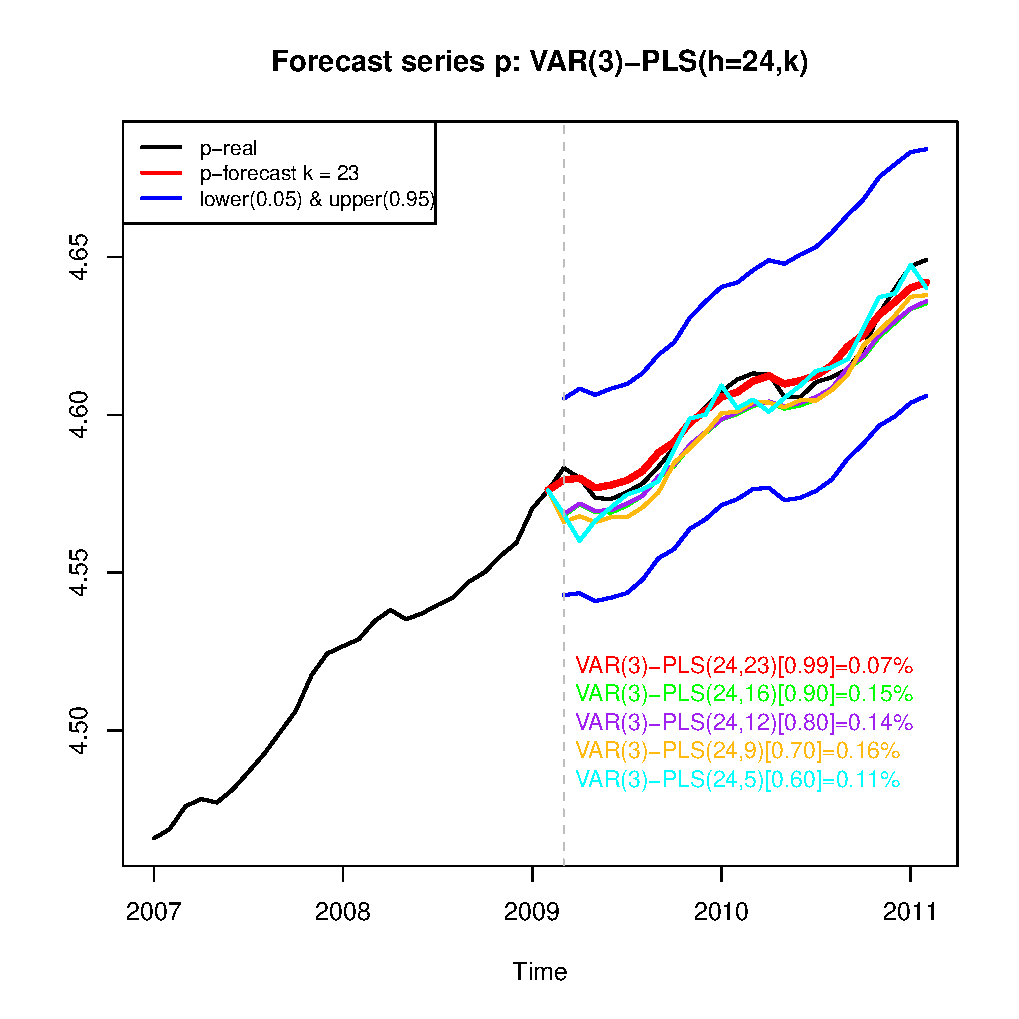
\includegraphics[scale=0.3]
      {figs/graph_2_v2.pdf}}
  \end{figure}
  \begin{footnotesize}
    \begin{itemize}
    \item Podemos observar que el valor real pr\'acticamente es el mismo
      que el pron\'ostico obtenido con un error absoluto promedio de
      0.11\%. Se muestran tambi\'en los intervalos de predicci\'on via
      Bootstrap que ``atrapan'' el valor real de la serie.
    \item En t\'erminos econ\'omicos, esta aproximaci\'on es competitiva.
    \end{itemize}
  \end{footnotesize}
\end{frame}

\begin{frame}{$VAR-PLS$}
  Notemos que, al ser un modelo multivariado se obtienen el resto de
  los pron\'osticos de las series, sin embargo, dado que el objetivo
  es predecir la serie de precios, no se considera relevante para este
  trabajo observar a detalle el comportamiento. No obstante, podemos
  comentar que el pron\'ostico con esta misma componente tuvo un error
  de 0.23\% para $m_0$, para $y$ 0.83\% y finalmente con un 5.84\% la
  tasa de inter\'es. 

  (NO LE ENTIENDO A ESTA REDACCI\'ON!!!!!!!!!)
\end{frame}

\begin{frame}{$VAR-PLS$}
  Para el Integral-VAR, los $VAR_J(P)$ \'optimos fueron los
  siguientes:
  \medskip

  \begin{footnotesize}
  \begin{tabular}{|l|c|c|c|c|}
    \hline
    Criterio & MAPE & MdAPE & RMSPE & RMdSPE \\
    \hline
    Estad\'istico & 0.29 & 0.30 & 0.33 & 0.30 \\
    Rezagos & 2 & 2& 2& 2 \\
    Estacionalidad & 10 & 10 & 10 & 10 \\
    Especificaci\'on & Constante y & Constante y & Constante y &
    Constante y \\
    & tendencia & tendencia & tendencia& tendencia \\
    \hline
  \end{tabular}
  \end{footnotesize}

  \begin{footnotesize}
  \begin{tabular}{|l|c|c|c|}
    \hline
    Criterio & MRAE & MdRAE & GMRAE \\
    \hline
    Estad\'istico & 0.24 & 0.22 & 0.18 \\
    Rezagos & 2& 2 & 3 \\
    Estacionalidad & 4 & 11 & 7 \\
    Especificaci\'on & Constante y & Constante y & Constante y \\
    & tendencia& tendencia& tendencia \\
    \hline
  \end{tabular}
  \end{footnotesize}
  \medskip

  Integrando los pron\'osticos y el intervalo de predicci\'on con su
  respectivo cuantil del 50\% para cada modelo y horizonte de
  pron\'ostico, obtenemos la siguiente figura:
\end{frame}

\begin{frame}{$VAR-PLS$}
  \begin{figure}[htbp]
    \center{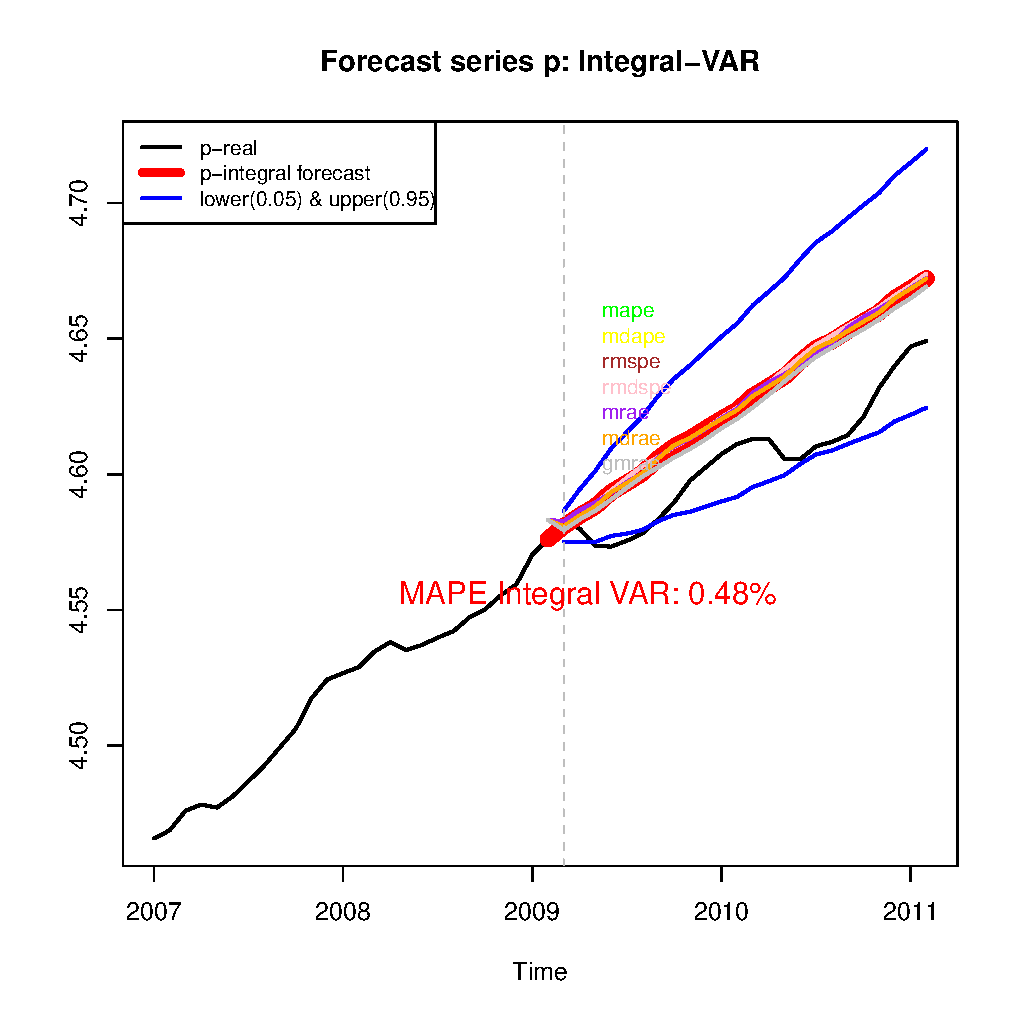
\includegraphics[scale=0.3]
      {figs/graph_3_v2.pdf}}
  \end{figure}
  \medskip

  Aunque en t\'erminos num\'ericos el error fue de 0.32\%, se observan
  grandes diferencias respecto al real observado, sobreestimando la
  inflaci\'on en cada uno de los casos. No obstante se decidi\'o
  realizarlo de esta manera para comparar las variables que
  intervienen en los pron\'osticos para ambas especificaciones.
\end{frame}

\begin{frame}{$VAR-PLS$}
  La siguiente figura muestra c\'omo se comport\'o cada componente
  respecto al Integral VAR:

  \begin{figure}[htbp]
    \center{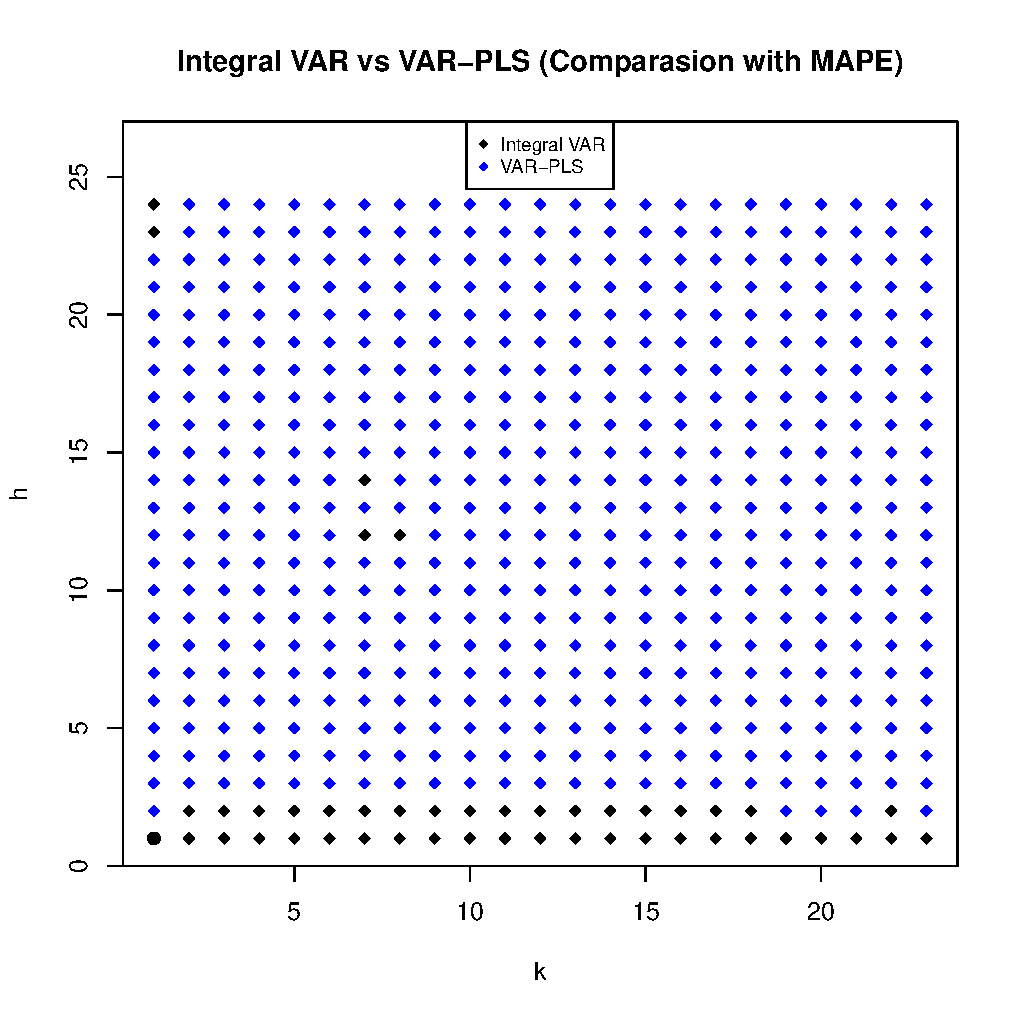
\includegraphics[scale=0.4]
      {figs/graph_4_v2.pdf}}
  \end{figure}
\end{frame}

\begin{frame}{$VAR-PLS$}
  Resulta interesante que en promedio, un 73.52\% de las veces
  fueron superior las componentes, y es l\'ogico que aquellas m\'as
  lejanas dejan de tener efectividad, dado que explican menos la
  variabilidad observada.
  \bigskip

  En otras palabras, la metodolog\'ia VAR-PLS resulta atractiva
  respecto a su competidor inmediate, que es un VAR enfocado a
  predecir.
 
\end{frame}

\begin{frame}{}
  \begin{block}{}
    \begin{center}
      \vspace{3mm}
      {\Large Conclusiones}
      \vspace{3mm}
    \end{center}
  \end{block}
\end{frame}

\begin{frame}{Conclusiones}
  \begin{itemize}
  \item En este trabajo se present\'o una alternativa para realizar
    pron\'osticos multivariados con el enfoque de explotar un
    conjunto de series de tiempo $y_{t+j}$ con $y_t$, aprovechando la
    naturaleza que tiene por construcci\'on la t\'ecnica de PLS,
    espec\'ificamente al momento de plantear un modelo lineal,
    situaci\'on que se presenta para el caso de un VAR.
  \item Se plante\'o un modelo que considera como principales fuentes
    inflacionarias un agregado monetario (billetes y monedas), tasas
    de inter\'es y una variable de ingreso, y se realizaron dos
    metodolog\'ias de pron\'ostico:
    \begin{itemize}
    \item un VAR-PLS cuyo orden $p$ est\'a dado por el criterio de FPE
      de un VAR, estimando todas las $pK$ componentes
    \item Finalmente, los intervalos de predicci\'on se hicieron
      mediante Bootstrap
    \end{itemize}
  \end{itemize}
  NO CREO QUE ESTE BIEN ESTA REDACCI\'ON... REVISAR!!!
\end{frame}

\begin{frame}{Conclusiones}
  De acuerdo a los resultados obtenidos, el VAR-PLS es una t\'ecnica
  atractiva de pron\'ostico multivariado.
  \medskip
  
  Como trabajo futuro queda:
  \begin{itemize}
  \item Incluir PLS en el ejercicio de cointegraci\'on, considerando
    las implicaciones te\'oricas.
  \item Construir modelos PLS-VAR que integren cada una de las
    componentes
  \item Comparar VAR-PLS y VAR que mezclen las variables que
    intervienen dentro de un pron\'ostico.
  \end{itemize}

\end{frame}

\begin{frame}{}
  \begin{block}{}
    \begin{center}
      \vspace{3mm}
      {\Large Gracias por su atenci\'on !}
      \vspace{3mm}
    \end{center}
  \end{block}
\end{frame}





\end{document}